\newcommand{\D}{$\Delta$}
\chapter{The language \D{}}

For the purposes of describing size-change termination we'll consider a
language \D{}. The following chapter describes the syntax and semantics of the
language.

\section{General properties}

The intent of the language is for it be used to explain concepts such as
size-change termination. One of the fundamental concepts required of the
language of application is that it's datatypes are well-founded. That is, any
subset $S$ of the range of values of some well-defined type has a value $s$
s.t. $\forall {s'\in S}\ s\leq s'$. This makes it ideal to chose some
oversimplistic data type structure rather than an army of basic types. Besides,
an apropriately defined basic data type should be able to represent arbitrarily
complex data values.

The language is initially first-order since the size-change termination
principle is first described for first-order programs later on in this work.
However, the language is designed so that it is easy to turn it into a
high-level language without much effort. This may prove necessary as we try to
expand size-change termination to higher-order programs.

The language is a call-by-value and purely functional to avoid any problems
that could arise from regarding lazy programs or where the notion of a global
state of the machine is relevant. Simply put, this is done to ensure elegance
of further proof with the help of the language.


\begin{frame}

\frametitle{\D{}, values and shapes}

\begin{columns}

\column{0.3\textwidth}
\begin{center}
$$b\in\mathbb{B}$$
\includegraphics[scale=0.5]{figures/value}
\end{center}

\column{0.3\textwidth}

\begin{center}
{\fontsize{40}{20}$\succ$}
\end{center}

\column{0.3\textwidth}

\begin{center}
$$s\in\mathbb{S}$$
\includegraphics[scale=0.5]{figures/shape}
\end{center}

\end{columns}

\end{frame}

\begin{frame}

\frametitle{\D{}, shapes and shapes}

\begin{columns}

\column{0.3\textwidth}
\begin{center}
$$s_1\in\mathbb{S}$$
\includegraphics[scale=0.5]{figures/shape}
\end{center}

\column{0.3\textwidth}

\begin{center}
{\fontsize{40}{20}$\succ$}
\end{center}

\column{0.3\textwidth}

\begin{center}
$$s_2\in\mathbb{S}$$
\includegraphics[scale=0.5]{figures/shape-2}
\end{center}

\end{columns}

\end{frame}

\begin{frame}

\frametitle{Disjoint shapes}

\begin{center}

$$s_1\cap s_2=\emptyset\quad\text{iff}\quad B_1\cap B_2=\emptyset$$

where

$$s_1,s_2\in\mathbb{S} \wedge B_1=\{b\mid b\in\mathbb{B} \wedge b\succ
s_1\}\wedge B_2=\{b\mid b\in\mathbb{B} \wedge b\succ s_2\}$$

\end{center}

\end{frame}

% TODO: All patterns now have a name.

\begin{frame}

\begin{center}

Given a shape $s_i\in\mathbb{S}$, we define the {\bf sibling set} $S^d_i$, to
be the pairwise disjoint set of shapes disjoint with $s_i$.

\end{center}

\end{frame}

\begin{frame}[fragile]

\begin{textblock}{1}(13.8,-3.5)$(35)$\end{textblock}

\begin{lstlisting}
data Pattern
  = PNil
  | PVariable String
  | PNode Pattern Pattern

getSiblings :: Pattern -> [Pattern]

getSiblings PNil =
  [PNode (PVariable "_") (PVariable "_")]

getSiblings (PVariable _) = []

getSiblings (PNode leftP rightP) =
  let
    leftS = getSiblings leftP
    rightS = getSiblings rightP
    leftInit = map (\s -> PNode leftP s) rightS
    rightInit = map (\s -> PNode s rightP) leftS
  in
    [PNil] ++
      leftInit ++ rightInit ++
      interleaveSiblings name leftS rightS
\end{lstlisting}

\end{frame}

\begin{frame}

\begin{align*}
T(1)&=4\\
T(n)&=1+T(n-1)+T(n-1)+T(n-1)\cdot T(n-1)
\end{align*}

\end{frame}

\section{Syntax}\label{section:d-syntax}

We describe the syntax of \D{} in terms of an extended Backus-Naur
form\footnote{The extension lends some constructs from regular expressions to
achieve a more concise dialect. The extension is described in detail in
\referToAppendix{ebnf}.}. This is a core syntax definition, and other, more
practical, syntactical features may be defined later on as needed. The initial
non-terminal is $\nonterm{program}$.

\begin{align}
\nonterm{program}\ ::=&\ \nonterm{clause}^*\ \nonterm{expression}\\
\nonterm{expression}\ ::=&\ \nonterm{element}\ (\ \term{.}\ \nonterm{expression}
\ )\ ?\\
\nonterm{element}\ ::=&\ \term{0}\ |\ \term{(}\ \nonterm{element}\ \term{)}\ |
\ \nonterm{name}\ |\ \nonterm{application}\\
\nonterm{application}\ ::=&\ \nonterm{name}
\ \nonterm{expression}^+\\
\nonterm{clause}\ ::=&\ \nonterm{name}\ \nonterm{pattern}^+
\ \term{:=}\ \nonterm{expression}\\
\label{nonterm-pattern}
\nonterm{pattern}\ ::=&\ \nonterm{pattern-element}\ (\ \term{.}
\ \nonterm{pattern}\ )\ ?\\
\label{nonterm-pattern-element}
\nonterm{pattern-element}\ ::=&\ \term{0}\ |\ \term{\_}\ |\ \term{(}
\ \nonterm{pattern}\ \term{)}\ |\ \nonterm{name}\\
\nonterm{name}\ ::=&\ [\term{a}\mathmono{-}\term{z}]
\ \left (\ [\term{-}\ \term{a}\mathmono{-}\term{z}]^*
\ [\term{a}\mathmono{-}\term{z}]\ \right )?
\end{align}

\begin{definition} \referToTable{sos-definitions} defines shorthands for
various language constructs. We'll often refer to these in further discussions.
Additionally, we'll let the atoms $0$ and $\_$ represent
themselves.\end{definition} 

\makeTable[h!]
{sos-definitions}
{Shorthands for various language constructs for use in latter discussions. We
provide shorthands for an instance, a list, and the space of a construct. For
instance, $x$ is some particular expression, $X$ is some particular list of
expressions, and $\mathbb{X}$ is the set of all possible expressions.}
{|l|c|c|c|}
{\textbf{Description}&\textbf{Instance}&\textbf{Finite list}&\textbf{Space}}
{
Expression & $x$ & $X$ & $\mathbb{X}$\\
Element (of an expression) & $e$ & $E$ & $\mathbb{E}$\\
Function & $f$ & $F$ & $\mathbb{F}$\\
Clause & $c$ & $C$ & $\mathbb{C}$\\
Pattern & $p$ & $P$ & $\mathbb{P}$\\
Value & $b$ & $B$ & $\mathbb{B}$\\
Name & $v$ & $V$ & $\mathbb{V}$\\
Program & $r$ & $R$ & $\mathbb{R}$
}

%\begin{definition} The \nonterm{expression} at the end of \nonterm{program} can
%be considered as the main clause of a program, which we'll refer to as
%$c_{main}$.\end{definition}

\begin{definition} For any given $v\in\mathbb{V}$ and $P\subset\mathbb{P}$,
we say that $v\in P$ if $v$ occurs in some $p\in P$.\end{definition}

\begin{definition}\label{definition:clause-tuple} A clause $c\in\mathbb{C}$ is
a tuple $\left\langle v,P,x \right\rangle$, where $v\in\mathbb{V}$ is the name
of the clause, $P\subset\mathbb{P}$ is a non-empty list of patterns of the
clause, and $x\in\mathbb{X}$ is the expression of the clause. $P$ is ordered by
occurrence of the patterns in the program text.\end{definition}

\begin{definition} We say that a clause $c= \left\langle v,P,x \right\rangle$
``accepts'' an argument list $B$ iff $|P|=|B|$ and $\forall\ \{i\mid 0\geq i <
|P|\}\ b_i\in B \wedge p_i\in P \wedge b_i\succ p_i$.\end{definition}

\begin{definition}\label{definition:function-tuple} A function $f\in\mathbb{F}$
is a tuple $\left\langle v,C \right\rangle$, where $v \in \mathbb{V}$ is the
name of the function, and $C\subset\mathbb{C}$ is the non-empty list of clauses
of the function. It must hold for $C$ that $\forall\ c\in C\
\left(c=\left\langle v_c, P_c, x_c \right\rangle \wedge v_c=v\right)$ and
$\forall\ c_1,c_2\in C\ \left(c_1=\left\langle v_1, P_1, x_1 \right\rangle
\wedge c_2=\left\langle v_2, P_2, x_2 \right\rangle \wedge |P_1|=|P_2|\right)$.
$C$ is ordered by occurrence of the clauses in the program
text.\end{definition}

\begin{definition} A signature of some function $f=\left\langle v, C
\right\rangle$ is the tuple $\left\langle v,|P| \right\rangle$, s.t.
$\forall\ c\in C_f\ |P_c|=|P|$. We'll adopt the Erlang notation when talking
about function signatures, i.e. if we have a function \mono{less} that takes in
two parameters, we'll refer to it as \mono{less/2}.\end{definition}

We assume for it to be fairly simple to construct the set $F$ of a given
program $r$ given the set of clauses $C$ derived during syntactic analysis of
the program text.

\begin{definition} A program $r$ is a tuple $\left\langle F,x \right\rangle$,
where $F\subset\mathbb{F}$ is the list of functions defined in program $r$, and
$x$ is the expression of program $r$.\end{definition}

\begin{definition}\label{definition:function-call} A function call is a tuple
$\left\langle v, X \right\rangle$, where $v\in\mathbb{V}$ is the name of the
callee, and $X\subset\mathbb{X}$ is a non-empty list of arguments for the
function call, ordered by occurrence of the expressions in the program
text.\end{definition}

0-ary clauses are disallowed to avoid having to deal with constants in general.
The term $\term{\_}$ in $\nonterm{pattern-element}$ is the conventional
wildcard operator; it indicates a value that won't used in the clause
expression, but some value has to be there for an argument to match the
pattern. Furthermore, as will be clear from the semantics, multiple occurrences
of \term{\_} in a clause pattern list does not indicate that the same value has
to be in place for each \term{\_}. 

\begin{definition} When describing various values and patterns in definitions,
theorems, proofs, etc. we'll sometimes make use of $\_$ to denote parts of the
value or pattern that are irrelevant to the said definition, theorem, proof,
etc.\end{definition}

% TODO this should be clear from the semantics.

% Multiple wildcards in the parameter list indicate possibly different value
% arguments, while multiple occurances of the same variable name in the parameter
% list are disallowed.

\subsection{Patterns constitute shapes}

The nonterminal declarations for patterns, in particular \ref{nonterm-pattern}
and \ref{nonterm-pattern-element}, indicate that a pattern are equatable to
shapes.

\begin{definition}\label{definition:pattern-corresponds-shape} The pattern
\term{0} corresponds to the leaf shape. The patterns \term{\_} and
\nonterm{name} correspond to triangle shapes. Any pattern \mono{a.b}
corresponds to the shape $a\cdot b$ iff the pattern \mono{a} corresponds to the
shape $a$ and the pattern \mono{b} corresponds to the shape
$b$.\end{definition}

\begin{definition}\label{definition:pattern-is-shape} $\forall\ p\in\mathbb{P}\
\forall\ s\in\mathbb{S}\ p=s$ iff $p$ corresponds to $s$ as by
\referToDefinition{pattern-corresponds-shape}.\end{definition}

\begin{definition} We overload the binary relation $\succ$ with the set\\
$\left\{ \left\langle p_1,p_2 \right\rangle\mid p_1,p_2\in\mathbb{P},
s_1,s_2\in\mathbb{S} \wedge p_1=s_1 \wedge p_2=s_2
\right\}$.\end{definition}

\subsection{Unary functions from multivariate functions}

The patterns of a clause as well as the arguments of a function call get
special treatment in \D{} in that they according to
\referToDefinition{clause-tuple} and \referToDefinition{function-call} are
ordered by their occurrence in the program text. This order is important to
make sure that the appropriate argument is matched against the appropriate
pattern. 

While this is setup is practical for the programmer, it is of no use to us due
to \referToTheorem{multivariate-to-unary}. In latter discussions, this
particular theorem allows us to keep to unary functions, and regard the
extension to multivariate functions as a fairly simple matter.

\begin{theorem}\label{theorem:multivariate-to-unary} Any multivariate function
in \D{} can be represented with a unary function.\end{theorem}

\begin{proof}

Given a multivariate function $f= \left\langle v,C \right\rangle$:

\begin{enumerate}

\item For each clause $c\in C$, where $c=\left\langle v,P,x \right\rangle$,
replace the pattern list $P$ with $P'=\{p\}$. Construct $p$ by initially
letting $p=0$, and folding left-wise over $P$, performing $p=p\cdot p'$ for
each $p'\in P$. 

\item For each call $\left\langle v, X\right\rangle$ to function $f$, replace
$X$ with the set $X'=\{x\}$, where $x$ has been constructed in a manner
equivalent to the pattern $p$ above.

\end{enumerate}

It is easy to see that both the constructed patterns and expressions are indeed
valid patterns and expressions, and that $f$ hence becomes a unary
function.\end{proof}

As this transformation is relatively simple to perform, we redefine the generic
clause tuple to have but one pattern in place of a list. 

\begin{definition}\label{definition:unary-clause} We redefine the clause $c$ to
be the tuple $\left\langle v,p,x\right\rangle$, where $v\in\mathbb{V}$ is the
name of the clause, $p\in\mathbb{P}$ is the pattern of the clause, and
$x\in\mathbb{X}$ is the expression of the clause.\end{definition}

\begin{definition}\label{definition:unary-function-call} We redefine a function
call to be the tuple $\left\langle v,x\right\rangle$, where $v\in\mathbb{V}$ is
the name of the callee, and $x\in\mathbb{X}$ is the argument to the (always
unary) callee.\end{definition}

\section{Semantics}\label{section:d-sos}

Revise the context of an expression within a function call, it should always be
the context upon entering the function call! Or even better, the context when
the function was defined!


\textbf{Perhaps pattern matching must be exhaustive in general.}

\textbf{Every subsequent definition must be strictly less specific than the former.}




In the following section we describe the semantics of \D{} using structured
operational semantics. The syntax used to define the reduction rules is largely
equivalent to the Aarhus report\cite{sos}, but differs slightly\footnote{The
syntax applied here is described in further detail in \referToAppendix{sos}.}.
The most notable about the syntax used here is the following:

\begin{itemize}

\item Rules should be read in increasing order of equation number.

\item If some rule with a lower equation number makes use of an undefined
reduction rule, it is because the reduction rule is defined under some higher
equation number.

\item Rules can be defined in terms of themselves, i.e. they can be recursive,
even mutually recursive.

\end{itemize}

The syntax aside, \referToTable{sos-definitions} defines a few lower-letter
shorthands for various constructs. Additionally, we'll let the capital
equivalents of these letters represent a sets of the respective construct, as
well as let the atoms $0$ and $\_$ represent themselves in the reduction rules.
It is also worth noting that $\forall\ v\in V\ :\ v\in \mathbb{B}$.

\makeTable[h!]
{sos-definitions}
{Overview of some of the shorthands used in this text. The column \textbf{A}
refers to all possible instances of the given construct, i.e.  $\mathbb{B}$
reffers to all constructable values in \D{}. The column \textbf{P} refers to
all the instances of the given construct in a given program, i.e. $N$ reffers
to all the names in a given program. The column \textbf{I} reffers to specific
instances of the given constructs, i.e. $x$ reffers to a particular
expression.}
{|l|c|c|c|}
{\textbf{Description}&\textbf{I}&\textbf{P}&\textbf{A}}
{
Expression & $x$ & $X$ & $\mathbb{X}$\\
Element (of an expression) & $e$ & $E$ & $\mathbb{E}$\\
Pattern & $p$ & $P$ & $\mathbb{P}$\\
Value(binary tree) & $b$ & $B$ & $\mathbb{B}$\\
Name & $n$ & $N$ & $\mathbb{N}$
}

\subsection{The memory model}\label{section:d-semantics-memory}

Memory is considered in terms of a set of value stacks, $\sigma$. Every stack
has a unique identifier $n\in N$, that is, each variable in a given program
gets a value stack. As we enter a new scope, we bind a variable to a value,
that is, we push that value on top of the corresponding stack. We pop the value
off the corresponding stack as we leave the scope at the entry to which the
variable was bound.

An expression at a certain scope depth only has access to variables at the same
scope depth. This is to ensure static scope. We won't adhere to this problem
explicitly in the semantics, but instead ask you to simply keep it in mind.

\subsubsection{Functions and variables}

Due to \D{} being a first-order language, we should make sure to separate the
function and variable spaces. We'll represent these by $\phi$ and $\gamma$,
respectively.

Whenever we use $\sigma$, $\phi$ or $\gamma$ in set notation, we imply the sets
of the names of functions and variables, and not the stacks themselves
corresponding to those names.  Hence, $\sigma=\phi\cup\gamma$, and to keep \D{}
first-order we add the limitation that $\phi\cap\gamma=\emptyset$.

\subsubsection{Making \D{} higher order}

The only change that this would require is to let $\phi=\gamma=\sigma$.

\subsection{Declaration}

A declaration with a name $n$, a \emph{non-empty} pattern
list $[p]$ and an expression $e$ is stored in the function space $\phi$:

\begin{equation}\label{sem:declaration}
{\displaystyle
  \left\langle \phi(n)\leftarrow \left\langle P, x\right\rangle\right\rangle
  \Rightarrow
  \phi'
\over\displaystyle
  \left\langle n, P, x, \phi\right\rangle
  \Rightarrow
  \phi'
}
\end{equation}

\subsection{Expression evaluation}

An expression $x$ is either the element $e$, or a construction of an element
$e'$ with another expression $x'$. That is, the binary infix operator $\cdot$
is right-associative, and has the following operational semantics:

\everymath{\displaystyle}

\begin{equation}
{\displaystyle
  \left\langle \proc{Single}, x,\sigma\right\rangle
  \rightarrow
  \left\langle v,\sigma\right\rangle
\vee
  \left\langle \proc{Chain}, x,\sigma\right\rangle
  \rightarrow
  \left\langle v,\sigma\right\rangle
\over\displaystyle
  \left\langle x,\sigma\right\rangle
  \rightarrow
  \left\langle v,\sigma\right\rangle
}
\end{equation}

\begin{equation}
{\displaystyle
  x\rightarrow e
\wedge
  \left\langle e,\sigma\right\rangle
  \rightarrow
  \left\langle v,\sigma\right\rangle
\over\displaystyle
  \left\langle \proc{Single}, x,\sigma\right\rangle
  \rightarrow
  \left\langle v,\sigma\right\rangle
}
\end{equation}

\begin{equation}
{\displaystyle
  x\Rightarrow e_1\cdot x_1
\wedge
  \left\langle e_1,\sigma\right\rangle
  \rightarrow
  \left\langle v_1,\sigma\right\rangle
\wedge
  \left\langle x_1,\sigma\right\rangle
  \rightarrow
  \left\langle v_2,\sigma\right\rangle
\over\displaystyle
  \left\langle \proc{Chain}, x, \sigma\right\rangle
  \rightarrow
  \left\langle v, \sigma\right\rangle
}
\quad(\text{where }v_1\cdot v_2=v)
\end{equation}

\subsection{Element evaluation}

According to the syntax specification, an element of an expression can either
be the atom $0$, or an application. We'd like to distinguish between variables
and functions, and we do that  

\begin{equation}
{\displaystyle
\left(
    e\Rightarrow 0
  \wedge
    v\equiv 0
\right)
\vee
{\displaystyle
    e\Rightarrow n
\over\displaystyle
    \beta(n)\Rightarrow v
}
\vee
{\displaystyle
    e\Rightarrow \left\langle n, X\right\rangle
\over\displaystyle
    \left\langle n,X,\sigma\right\rangle
    \Rightarrow
    \left\langle v,\sigma\right\rangle
}
\over\displaystyle
\left\langle e,\sigma\right\rangle
\Rightarrow
\left\langle v,\sigma\right\rangle
}
\end{equation}

\subsection{Function application}

\begin{equation}
{\displaystyle
{\displaystyle
{\displaystyle
  \left\langle n, \phi\right\rangle
  \Rightarrow
  \left\langle P, x, \phi\right\rangle
\over\displaystyle
  \left\langle P, X, \sigma\right\rangle
  \Rightarrow
  \sigma'
}
\over\displaystyle
  \left\langle x, \sigma'\right\rangle
  \Rightarrow
  \left\langle v,\sigma'\right\rangle
}
\over\displaystyle
    \left\langle n,X,\sigma\right\rangle
    \Rightarrow
    \left\langle v,\sigma\right\rangle
}
\end{equation}

\subsection{Pattern matching}

\begin{equation}
{\displaystyle
{\displaystyle
  \left\langle P_{head}, X_{head}, \sigma\right\rangle
  \Rightarrow
  \sigma''
\over\displaystyle
  \left\langle P_{tail}, X_{tail}, \sigma''\right\rangle
  \Rightarrow
  \sigma'
}
\over\displaystyle
  \left\langle P, X, \sigma\right\rangle
  \Rightarrow
  \sigma'
}
\end{equation}

\begin{equation}
{
  \left\langle\proc{I}, p,x,\sigma\right\rangle
  \Rightarrow
  \left\langle p',x',\sigma'\right\rangle
\vee
  \left\langle\proc{Z}, p,x,\sigma\right\rangle
  \Rightarrow
  \left\langle p',x',\sigma'\right\rangle
\vee
  \left\langle\proc{N}, p,x,\sigma\right\rangle
  \Rightarrow
  \left\langle p',x',\sigma'\right\rangle
\vee
  \left\langle\proc{P}, p,x,\sigma\right\rangle
  \Rightarrow
  \left\langle p',x',\sigma'\right\rangle
}\over{
  \left\langle p, x, \sigma\right\rangle
  \Rightarrow
  \left\langle p', x', \sigma'\right\rangle
}
\end{equation}

For the sake of an elegant notation, we'll override the function $\cdot$ for
patterns.

\begin{definition}

A pattern is an unlabeled of binary tree which is either empty or consists of
an unlabeled node with a $0$, $\_$, name, or a pattern as it's left and right
child. 

\end{definition}

\begin{definition}

Let the set of all possible patterns be denoted by $\mathbb{P}$.

\end{definition}

\begin{definition}

The function $\cdot
:\mathbb{P}\times\mathbb{P}\rightarrow\mathbb{P}$ constructs a pattern node with the
two arguments as it's left and right child, respectively. 

\end{definition}

\begin{equation}
{
    p\Rightarrow \_\cdot p'
  \wedge
    x\Rightarrow e\cdot x'
  \wedge
    \sigma\Rightarrow\sigma'
}\over{
  \left\langle\proc{Underscore}, p,x,\sigma\right\rangle
  \Rightarrow
  \left\langle p',x',\sigma'\right\rangle
}
\end{equation}

\begin{equation}
{
    p\Rightarrow 0\cdot p'
  \wedge
    x\Rightarrow e\cdot x'
  \wedge
    \sigma\Rightarrow\sigma'
}\over{
  \left\langle\proc{Zero}, p,x,\sigma\right\rangle
  \Rightarrow
  \left\langle p',x',\sigma'\right\rangle
}
\end{equation}


\begin{equation}
{\displaystyle
{\displaystyle
{\displaystyle
    p\Rightarrow n\cdot p'
  \wedge
    x\Rightarrow e\cdot x'
\over\displaystyle
    \left\langle e,\sigma\right\rangle
    \Rightarrow
    \left\langle v,\sigma\right\rangle
}\over\displaystyle
    \left\langle\sigma(n)\leftarrow v\right\rangle
    \Rightarrow
    \sigma'
}\over\displaystyle
  \left\langle\proc{Name}, p,x,\sigma\right\rangle
  \Rightarrow
  \left\langle p',x',\sigma'\right\rangle
}
\end{equation}

\begin{equation}
{\displaystyle
{\displaystyle
    p\Rightarrow p''\cdot p'  
  \wedge
    x\Rightarrow x''\cdot x'
\over\displaystyle
  \left\langle p'', x'', \sigma\right\rangle
  \Rightarrow
  \sigma'
}
\over\displaystyle
  \left\langle\proc{Pattern}, p,x,\sigma\right\rangle
  \Rightarrow
  \left\langle p',x',\sigma'\right\rangle
}
\end{equation}

\input{language/input}
\section{Size}

For the purposes of talking about size-change termination, we also need to
define the notion of size, and be sure to do so in such a way so that all
possible data values are well-founded.

\begin{definition}\label{definition:size}

Size of a value in \D{} is the number of nodes in the tree representing
that value.

\end{definition}

The ``well-foundedness'' of \D{}'s data values, given such a definition can be
argued for by proving a bijective relation between $\mathbb{B}$ and
$\mathbb{N}$. This would imply that we can define the relation $<$ on \D{}'s
data values, which we know to be well-founded.

We start by formally proving that \referToDefinition{size} yields a many-to-one
mapping of \D{}'s data values to the natural numbers.

First, we prove, by induction, that any natural number can be represented in
\D{}:

\begin{proof}\ \\

\begin{description}[\setleftmargin{70pt}\setlabelstyle{\bf}]

\item [Base] The atom $0$ has no nodes, and hence represents the value $0$.

\item [Assumption] If we can represent the $n\in\mathbb{N}$ in \D{}, then
we can also represent the number $n+1\in\mathbb{N}$. 

\item [Induction] Let $n$ be represented by some binary tree $A$, then $n+1$
can be represented by $0\cdot A$. 

\end{description}

\end{proof}

Second, we prove, also by induction, that any value in \D{} has one and only
one representation in $\mathbb{N}$.

\begin{proof}\ \\

\begin{description}[\setleftmargin{70pt}\setlabelstyle{\bf}]

\item [Base] The atom $0$ has no nodes, and hence corresponds only to the value
$0$.

\item [Assumption]

\begin{enumerate}

\item If the binary tree $A$ has only one representation $n\in\mathbb{N}$, then
$\left|0\cdot A\right|\equiv n+1$ and $\left|A\cdot 0\right|\equiv n+1$.

\item If the binary tree $A$ has only one representation $n\in\mathbb{N}$, and
the binary tree $B$ has only one representation $m\in\mathbb{N}$, then
$\left|A\cdot B\right|\equiv n+m+1$ and $\left|B\cdot A\right|\equiv n+m+1$.

\end{enumerate}

\item [Induction]

By definition of the binary function $\cdot$, any given node $A$ with left
child $A_{left}$ and right child $A_{right}$ has the size:

$$\left|A\right|=1+\left|A_{left}\right|+\left|A_{right}\right|$$

Hence, any value in \D{} must have one and only one representation in
$\mathbb{N}$.

\end{description}

\end{proof}

\referToDefinition{size} \emph{almost} allows us to devise an algorithm to
compare the sizes of data values. The problem withstanding is that two
different values can have rather diverging tree representations. Hence,
comparing them, using only the operations defined in \referToSection{d-sos}, is
seemingly impossible unless we initially, or along the way, transform the
binary trees being compared into some sort of a \emph{standard representation}.
We'll define this representation, recursively, as follows:

\begin{definition}\label{definition:standard-representation}

A binary tree in standard representation is a binary tree that either is a leaf
or a node having a leaf as its left child and a binary tree in standard
representation as its right child.

\end{definition}

Intuitively, a binary tree in standard representation is just a tree that only
descends along the right side. Comparing the sizes of two trees in this
representation is just a matter of walking the descending in the two trees
simultaneously, until one of them, or both, bottom out. If there is a tree that
bottoms out strictly before another, that is the lesser tree by
\referToDefinition{size}. \referToFigure{standard-representation} showcases
some examples.

\begin{figure}[htbp!]
\centering
\subfigure[{Not in standard representation}]
{
  \includegraphics[scale=1]{figures/first-non-standard}
}
\subfigure[{Not in standard representation}]
{
  \includegraphics[scale=1]{figures/second-non-standard}
}
\subfigure[{Standard representation}]
{
  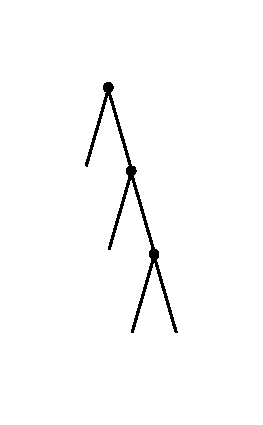
\includegraphics[scale=1]{figures/standard}
}
\caption[]{Three trees of various shapes but equal size.}
\label{figure:standard-representation}
\end{figure}

\subsection{\mono{normalize/1}}

\begin{verbatim}
normalize a = normalize-aux a 0 0

normalize-aux 0     0     an = an
normalize-aux 0     bl.br an = normalize-aux bl br    an
normalize-aux 0.ar  b     an = normalize-aux ar b     0.an
normalize-aux al.0  b     an = normalize-aux al b     0.an
normalize-aux al.ar b     an = normalize-aux ar al.b  0.an

\end{verbatim}

\subsubsection{Correctness}

\mono{normalize/1} makes use of an auxiliary procedure, \mono{normalize-aux/3},
for which we can provide the following argument descriptions:

\begin{enumerate}

\item The tree to be normalized.

\item An auxiliary tree.

\item A normalized tree.

\end{enumerate} 

The idea of the algorithm is to move right-wise down the tree to be normalized,
constructing an auxiliary tree containing all left-wise child nodes, if any.

The return value is the normalized tree, i.e. the third argument. Hence, we
must increase the size of the normalized tree each time we move right-wise down
the tree to be normalized.

Once we reach the right-most leaf of the tree to be normalized we return the
normalized tree if the auxiliary tree is empty. Otherwise, we normalize the
right child of the auxilary tree, with the left child of the auxiliary as the
new auxiliary tree, and the normalized tree constructed thus far as the initial
normalized tree.

\subsubsection{Time complexity}

Coming soon..

\subsubsection{Space complexity}

Coming soon..

\subsection{\mono{less/2}}\label{section:d-size-less}

We'll define the function \mono{normalize/1} further below to transform any
\D{} value into its standard representation. For now we'll assume that we have
such a function in scope and define \mono{less/2} for determining whether the
value of the first argument is strictly less than the value of the second
argument.

In order to define such a boolean-valued function we need a convention for
representing the boolean values $true$ and $false$ in \D{}. We'll adopt the
C-like convention:

\begin{definition}

A $false$ value is represented by a leaf tree. A $true$ value is represented by
a non-leaf tree, i.e. a node.

\end{definition}

We're now ready to define the function \mono{less/2}:

\begin{lstlisting}[label={listing:d-less},caption={A definition of the \mono{less/2} function.}]
less a b := normalized-less (normalize a) (normalize b)

normalized-less 0 b := b
normalized-less _ 0 := 0
normalized-less _.a _.b := normalized-less a b
\end{lstlisting}

\subsubsection{Correctness}

\begin{proof}

Given \referToDefinition{standard-representation}, and the assumption that
$\proc{Normalize}(A)$ computes the standard representation of $A$, we know the
following:

\begin{enumerate}

\item $\left|A\right|\equiv\left|\proc{Normalize}(A)\right|$.

\item We'll walk through all the nodes if we perform a recursive
right-child-walk starting at $A$.

\item The same holds for $B$.

\end{enumerate}

It is also easy to see from lines
\ref{normalized-less-init-start}:\ref{normalized-less-init-end} that
$\proc{NormalizedLess}$ stops as soon as we reach the ``bottom'' of either $A$
or $B$.

Given \referToDefinition{size}, $A<B$ iff it bottoms out before $B$, that is,
we reach an instance of the recursion where both $IsLeaf(A)$ and $IsNode(B)$
hold.  In all other cases $A\geq B$, the cases specifically are:

\begin{itemize}

\item $IsLeaf(A)$ and $IsLeaf(B)$, then $\left|A\right|\equiv \left|B\right|$.

\item $IsNode(A)$ and $IsLeaf(B)$, then $\left|A\right|>\left|B\right|$

\end{itemize}

Last but not least, due to all data values being finite, eventually one of the
trees does bottom out.

\end{proof}

\subsubsection{Time complexity}

Given that the binary trees $A$ and $B$ are in standard representation when we
enter the auxiliary procedure, $\proc{NormalizedLess}$, it is fairly easy to
get an upper bound on the running time of $\proc{NormalizedLess}$ itself.

Indeed, the running time of $\proc{NormalizedLess}$ itself is
$O\left(\proc{Max}\left(\left|A\right|,\left|B\right|\right)\right)$, since we
just walk down the trees until one of them bottoms out. 

We haven't yet defined the procedure $\proc{Normalize}$ yet. Hence, the only
thing that we can say about the running time of $\proc{Less}$ in general is
that it is $O\left(\proc{Normalize}(A) + \proc{Normalize}(B) +
\proc{Max}\left(\left|A\right|,\left|B\right|\right) \right)$.

\subsubsection{Space complexity}

Coming soon..

\section{Built-in high-order
functions}\label{section:language-higher-order-built-ins}

Although \mono{D} is initially a first-order language, we will ignore that
limitation for a bit and define a few higher-order functions to provide some
syntactical sugar to the language. Beyond the discussion in this section, these
higher-order functions should be regarded as \mono{D} built-ins.

\subsubsection{Branching}

In the following definition, the variable names \mono{true} and \mono{false}
refer to expressions to be executed in either case.

\begin{verbatim}
if 0 _ false := false
if _._ _ true := true
\end{verbatim}

As you can see, we employ the C convention that any value other than $0$ is a
``truthy'' value, and the expression \mono{true} is returned.

Although the call-by-value nature of the language does not allow for
short-circuiting the if-statements defined in such a way, this shouldn't be any
impediment to further analysis.

\subsection{Boolean operations}

\begin{verbatim}
and _._ _._ = 0.0
and _ _ = 0

or 0 0 = 0
or _ _ = 0.0
\end{verbatim}


\section{Sample programs}\label{section:d-samples}

As an illustration of the language syntax, take a look at the programs in
\referToListing{reverse}, \referToListing{fibonacci} and
\referToListing{ackermann}.

\begin{lstlisting}[label=listing:reverse,
  caption={A program that reverses the order of the nodes of some supplied tree.}]
reverse 0 := 0
reverse left.right := (reverse right).(reverse left)

reverse input
\end{lstlisting}

\begin{lstlisting}[label=listing:fibonacci,
  caption={A program that computes the $n^{th}$ fibonacci when supplied with some $n$.}] 
fibonacci n = fibonacci-aux (normalize n) 0 0

fibonacci-aux 0 x y := 0
fibonacci-aux 0.0 x y := y
fibonacci-aux 0.n x y := fibonacci-aux n y (add x y)

fibonacci input
\end{lstlisting}

\begin{lstlisting}[label=listing:ackermann,
  caption={The Ackermann-P\'eter function.}]
ackermann 0 n := 0.n
ackermann a.b 0 := ackermann (decrease a.b) 1
ackermann a.b c.d := ackermann (decrease a.b) (ackermann a.b (decrease c.d))

ackermann input input
\end{lstlisting}

